% sec_4_4_dynamics.tex — Динамика смазочного слоя

Разделы~4.1--4.3 рассматривали нелинейные эффекты применительно к~стационарному вращению вала при~фиксированном положении его~центра. В~реальных условиях эксплуатации вал совершает малые колебания относительно равновесного положения под~действием дисбаланса, переходных нагрузок и~гидродинамических возмущений. Реакция смазочного слоя на~эти~колебания описывается линеаризованными коэффициентами жёсткости и~демпфирования, которые определяют динамические свойства опорного узла и~устойчивость роторной системы в~целом~\cite{goodwin1997,jang1999,sayed2022,muszynska1988,weissbacher2014}.

\textit{Линеаризация по~малым возмущениям положения вала.}
Равновесное положение центра вала характеризуется координатами~$(x_0,\,y_0)$ или, эквивалентно, эксцентриситетом~$\varepsilon_0$ и~углом нагружения~$\psi_0$. При~малом возмущении центр вала смещается в~положение~$(x_0 + \xi,\; y_0 + \eta)$, где~$|\xi|,\,|\eta| \ll c$.

Безразмерная толщина зазора с~учётом возмущения записывается в~виде
\begin{equation}
  H(\theta,\,t) = H_0(\theta)
    - \bar{\xi}(t)\,\cos\theta
    - \bar{\eta}(t)\,\sin\theta,
  \label{eq:H_perturbed}
\end{equation}
\begin{conditions}
$H_0(\theta) = 1 + \varepsilon_0\cos\theta$ -- равновесный зазор радиального подшипника~\eqref{eq:journal_h};\\
$\bar{\xi} = \xi/c$,\; $\bar{\eta} = \eta/c$ -- безразмерные составляющие возмущения положения центра вала.
\end{conditions}
Давление разлагается по~малому параметру:
\begin{equation}
  P = P_0
    + \bar{\xi}\,P_{\xi}
    + \bar{\eta}\,P_{\eta}
    + \dot{\bar{\xi}}\,P_{\dot\xi}
    + \dot{\bar{\eta}}\,P_{\dot\eta}
    + \ldots
  \label{eq:P_expansion}
\end{equation}
Здесь~$P_0$~-- стационарное давление (главы~5--7); поля~$P_{\xi}$, $P_{\eta}$, $P_{\dot\xi}$, $P_{\dot\eta}$ находятся из~линеаризованных уравнений Рейнольдса с~правыми частями, получаемыми дифференцированием~\eqref{eq:reynolds_nondim} по~соответствующим переменным.

В~постановке JFO~\eqref{eq:jfo_conservation} граница кавитационной области при~возмущении может смещаться. В~первом приближении используется допущение о~фиксированной кавитационной области (\textit{frozen cavitation}): граница~$\partial\Omega_{\mathrm{cav}}$ определяется по~равновесному полю~$P_0$. Альтернативные подходы и~их~сравнение рассматриваются в~главе~8.

\textit{Матрицы жёсткости и~демпфирования смазочного слоя.}
Линеаризация гидродинамической силы приводит к~выражению
\begin{equation}
  \begin{pmatrix} \Delta F_x \\ \Delta F_y \end{pmatrix}
  = -\mathbf{K}
  \begin{pmatrix} \bar\xi \\ \bar\eta \end{pmatrix}
  - \mathbf{C}
  \begin{pmatrix} \dot{\bar\xi} \\ \dot{\bar\eta} \end{pmatrix},
  \label{eq:linearized_force}
\end{equation}
где~компоненты матриц жёсткости~$\mathbf{K}$ и~демпфирования~$\mathbf{C}$ определяются как
\begin{equation}
  K_{ij} = -\frac{\partial F_i}{\partial \bar{q}_j}\bigg|_0, \qquad
  C_{ij} = -\frac{\partial F_i}{\partial \dot{\bar{q}}_j}\bigg|_0,
  \quad i,j \in \{x,\,y\},
  \label{eq:KC_def}
\end{equation}
а~численное вычисление выполняется интегрированием возмущённых давлений по~области смазочного слоя:
\begin{equation}
  K_{xx} = -\iint_\Omega P_{\xi}\,\cos\theta\;d\theta\,dZ, \qquad
  K_{xy} = -\iint_\Omega P_{\eta}\,\cos\theta\;d\theta\,dZ,
  \label{eq:K_integrals}
\end{equation}
аналогично для~$K_{yx}$, $K_{yy}$ и~для~$C_{xx}$, $C_{xy}$, $C_{yx}$, $C_{yy}$ через~$P_{\dot\xi}$, $P_{\dot\eta}$.

Детерминированные микроструктуры изменяют стационарное поле~$P_0$ и~возмущённые поля~$P_{\xi}$, $P_{\eta}$, $P_{\dot\xi}$, $P_{\dot\eta}$, а~следовательно, компоненты~$K_{ij}$ и~$C_{ij}$. Это~является основным каналом влияния текстуры поверхности на~динамические характеристики опорного узла. Матрицы~$\mathbf{K}$ и~$\mathbf{C}$ в~общем случае несимметричны: перекрёстные коэффициенты~$K_{xy} \neq K_{yx}$, $C_{xy} \neq C_{yx}$, что~обусловлено вращательным характером течения смазки и~является принципиальным отличием подшипников скольжения от~упругих опор.

\textit{Критерии устойчивости роторно-подшипниковой системы.}
Уравнение движения ротора массой~$M$ в~двухкоординатной ($2$DOF) модели записывается в~виде
\begin{equation}
  M\,\ddot{\mathbf{q}} + \mathbf{C}\,\dot{\mathbf{q}} + \mathbf{K}\,\mathbf{q} = 0,
  \qquad \mathbf{q} = (\bar\xi,\,\bar\eta)^T.
  \label{eq:rotor_eom}
\end{equation}
Переход к~переменным состояния~$\mathbf{u} = (\mathbf{q},\,\dot{\mathbf{q}})^T$ приводит систему к~стандартной форме
\begin{equation}
  \dot{\mathbf{u}} = \mathbf{A}\,\mathbf{u}, \qquad
  \mathbf{A} =
  \begin{pmatrix}
    \mathbf{0} & \mathbf{I} \\
    -M^{-1}\mathbf{K} & -M^{-1}\mathbf{C}
  \end{pmatrix}.
  \label{eq:state_matrix}
\end{equation}
Система асимптотически устойчива тогда и~только тогда, когда все~собственные значения~$\lambda_k$ матрицы~$\mathbf{A}$ имеют отрицательную вещественную часть: $\mathrm{Re}(\lambda_k) < 0$ для~всех~$k$. Если~хотя~бы~для~одного~$k$ выполняется~$\mathrm{Re}(\lambda_k) > 0$, система неустойчива; граничный случай~$\max_k \mathrm{Re}(\lambda_k) = 0$ соответствует порогу устойчивости (критической скорости).

Формулы для~критических скоростей и~интегральных критериев устойчивости зависят от~конкретной модели ротора (масса, жёсткость вала, гироскопика) и~в~данном разделе не~приводятся; количественный пример применительно к~подшипнику центробежного насоса рассматривается в~главе~8.

Общая схема линеаризованной модели сил смазочного слоя
приведена на рисунке~\ref{fig:linearized_forces}.

\begin{figure}[!ht]
\centering
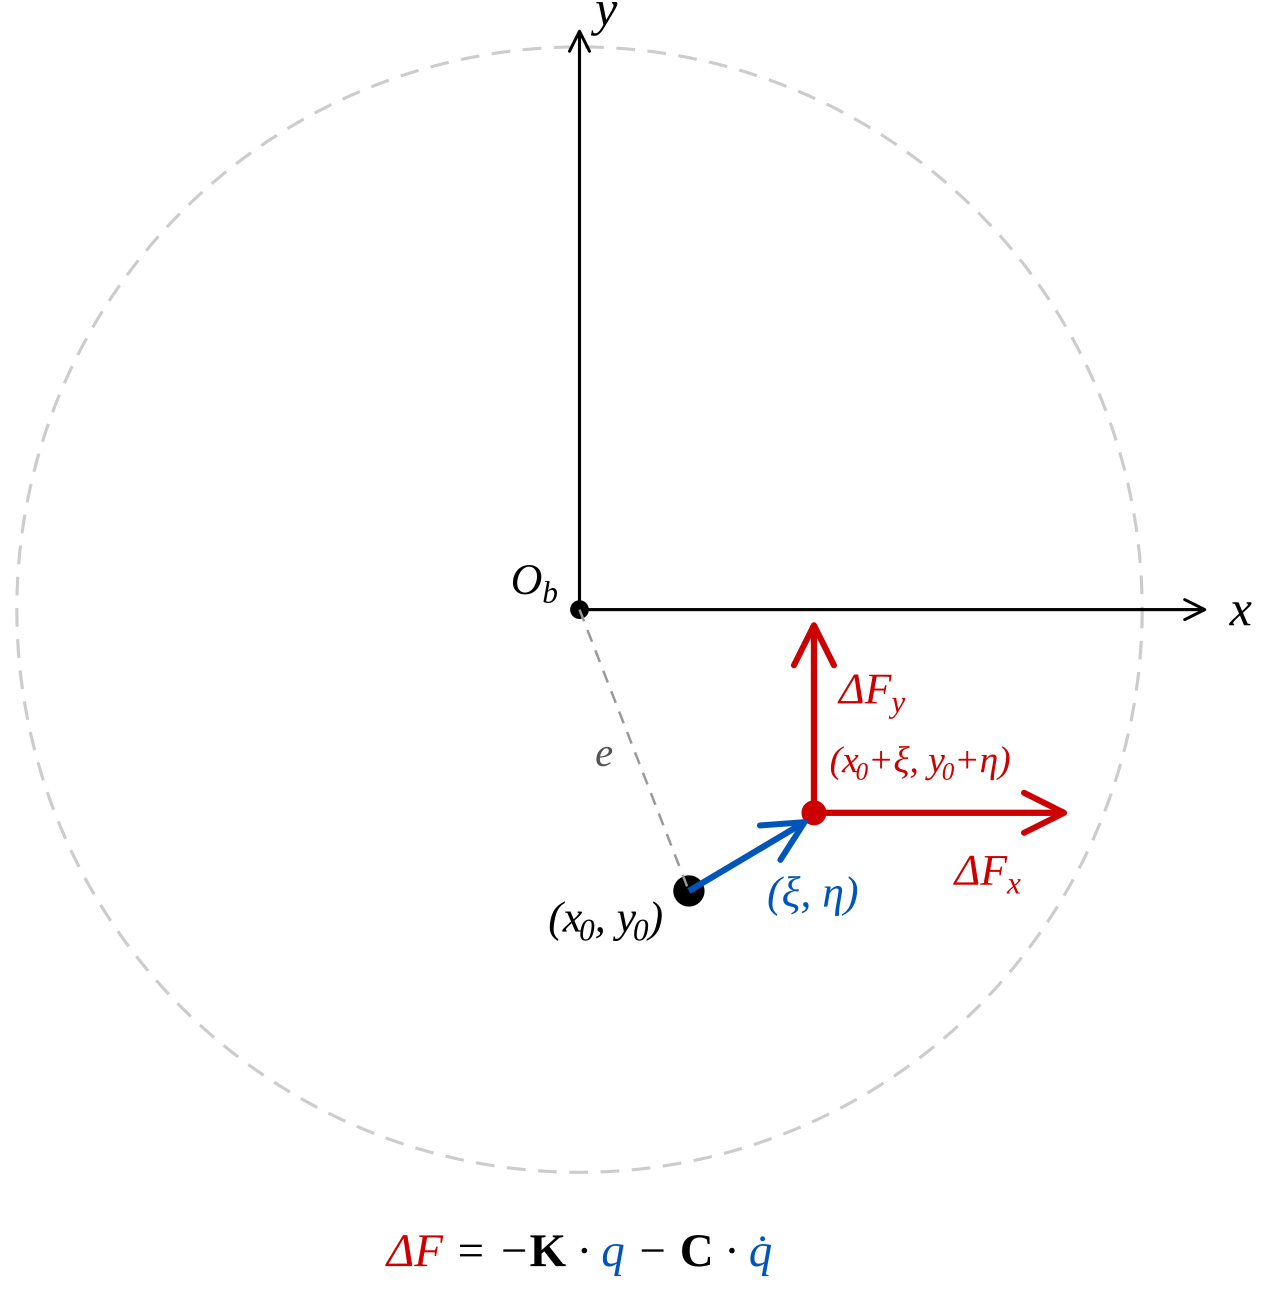
\includegraphics[width=\textwidth,height=0.9\textheight,keepaspectratio]{figures/ch04/fig_4_5.png}
\caption{Линеаризованная модель сил смазочного слоя при малых колебаниях вала}
\label{fig:linearized_forces}
\end{figure}

\FloatBarrier

Линеаризованные коэффициенты жёсткости и~демпфирования
полностью определяются стационарным и~возмущёнными полями
давления; влияние детерминированных микроструктур на~эти
коэффициенты и~устойчивость роторной системы количественно
исследуется в~главе~8.

\textit{Физический смысл прямых и перекрёстных коэффициентов.}
Физический смысл коэффициентов целесообразно пояснить
на примере радиального подшипника. Прямые
жёсткости $K_{xx}$, $K_{yy}$ характеризуют возвращающую силу
при смещении вала вдоль соответствующей оси: $K_{xx} > 0$
означает, что смещение по~$x$ порождает силу, направленную
против смещения (упругоподобное поведение). Прямые
демпфирования $C_{xx}$, $C_{yy}$ определяют диссипативные
силы, противодействующие скорости вала: $C_{xx} > 0$ означает
торможение при движении по~$x$.

Перекрёстные коэффициенты~$K_{xy}$, $K_{yx}$, $C_{xy}$,
$C_{yx}$ описывают связь между двумя направлениями движения.
Для подшипника скольжения перекрёстные жёсткости обычно имеют
противоположные знаки: $K_{xy} > 0$, $K_{yx} < 0$. Это
соответствует циркуляторным силам~-- силам, перпендикулярным
скорости; они не совершают работы в среднем за период,
но могут раскачивать орбиту. Именно наличие циркуляторной пары
$K_{xy} \neq 0$, $K_{yx} \neq 0$ является физическим
механизмом нестабильности типа «вихревая прецессия»
(oil whirl), характерной для подшипников скольжения при
больших скоростях.

\textit{Механизм нестабильности типа вихревой прецессии и~роль текстуры.}
Нестабильность типа oil whirl (вихревая прецессия) возникает, когда циркуляторные силы от~перекрёстных жёсткостей превышают диссипацию от~прямых демпфирований. В~линейной модели~\eqref{eq:rotor_eom} критерий потери устойчивости формулируется через знак~$\mathrm{Re}(\lambda)$, однако физически механизм можно описать следующим образом. При~смещении центра вала по~направлению~$x$ возникает сила~$K_{yx}\,\xi$ в~направлении~$y$ (при~$K_{yx} < 0$ --- это сила, перпендикулярная смещению и~направленная по~вращению). Эта сила раскручивает орбиту вала, постепенно увеличивая её~радиус. Прямое демпфирование~$C_{xx}$, $C_{yy}$ противодействует этому процессу, но~при~достаточно высоких скоростях вращения (и~соответственно высоком давлении смазки) циркуляторная сила превышает диссипацию, и~орбита начинает раскручиваться неограниченно~--- наступает нестабильность.

Детерминированные микроструктуры влияют на~этот баланс через~два канала. С~одной стороны, они изменяют равновесное поле давления~$P_0$ и~тем самым модифицируют все~восемь коэффициентов. С~другой стороны, они изменяют геометрию зазора~$H$, что непосредственно сказывается на~возмущённых полях~$P_\xi$, $P_\eta$, $P_{\dot\xi}$, $P_{\dot\eta}$. Результирующий эффект определяется расположением и~геометрией лунок: текстура во~входной части клина может усиливать прямые жёсткости и~улучшать демпфирование, тогда как~текстура в~зоне убывающего давления оказывает обратное действие~--- это качественно согласуется с~результатами глав~5--7 по~статическому анализу.

\textit{Ограниченность линейной модели.}
Линейная модель~\eqref{eq:rotor_eom} применима только при~малых амплитудах колебаний~$|\xi|, |\eta| \ll c$. При~амплитудах, сопоставимых с~зазором~$c$, нелинейные эффекты становятся существенными: форма орбиты отклоняется от~эллиптической, спектр колебаний обогащается гармониками, а~в~некоторых случаях возникают квазипериодические или хаотические режимы движения. В~этих условиях применение линейных коэффициентов~$K_{ij}$, $C_{ij}$ приводит к~качественно неверным предсказаниям. Полноценный нелинейный анализ требует численного интегрирования уравнений движения с~пересчётом поля давления на~каждом временном шаге, что в~несколько порядков увеличивает вычислительные затраты. Для~целей данной монографии рассматривается только линейная модель; проверка её~применимости выполняется через сравнение максимальных амплитуд с~зазором~$c$ (глава~8).

\textit{Механизм нестабильности типа вихревой прецессии и~роль текстуры.}
Нестабильность типа oil whirl (вихревая прецессия) возникает, когда циркуляторные силы от~перекрёстных жёсткостей превышают диссипацию от~прямых демпфирований. В~линейной модели~\eqref{eq:rotor_eom} критерий потери устойчивости формулируется через знак~$\mathrm{Re}(\lambda)$, однако физически механизм можно описать следующим образом. При~смещении центра вала по~направлению~$x$ возникает сила~$K_{yx}\,\xi$ в~направлении~$y$ (при~$K_{yx} < 0$~--- это сила, перпендикулярная смещению и~направленная по~вращению). Эта сила раскручивает орбиту вала, постепенно увеличивая её~радиус. Прямое демпфирование~$C_{xx}$, $C_{yy}$ противодействует этому процессу, но~при~достаточно высоких скоростях вращения (и~соответственно высоком давлении смазки) циркуляторная сила превышает диссипацию, и~орбита начинает раскручиваться неограниченно~--- наступает нестабильность.

Детерминированные микроструктуры влияют на~этот баланс через~два канала. С~одной стороны, они изменяют равновесное поле давления~$P_0$ и~тем самым модифицируют все~восемь коэффициентов. С~другой стороны, они изменяют геометрию зазора~$H$, что непосредственно сказывается на~возмущённых полях~$P_\xi$, $P_\eta$, $P_{\dot\xi}$, $P_{\dot\eta}$. Результирующий эффект определяется расположением и~геометрией лунок: текстура во~входной части клина может усиливать прямые жёсткости и~улучшать демпфирование, тогда как~текстура в~зоне убывающего давления оказывает обратное действие~--- это качественно согласуется с~результатами глав~5--7 по~статическому анализу.

\textit{Ограниченность линейной модели.}
Линейная модель~\eqref{eq:rotor_eom} применима только при~малых амплитудах колебаний~$|\xi|, |\eta| \ll c$. При~амплитудах, сопоставимых с~зазором~$c$, нелинейные эффекты становятся существенными: форма орбиты отклоняется от~эллиптической, спектр колебаний обогащается гармониками, а~в~некоторых случаях возникают квазипериодические или хаотические режимы движения. В~этих условиях применение линейных коэффициентов~$K_{ij}$, $C_{ij}$ приводит к~качественно неверным предсказаниям. Полноценный нелинейный анализ требует численного интегрирования уравнений движения с~пересчётом поля давления на~каждом временном шаге, что в~несколько порядков увеличивает вычислительные затраты. Для~целей данной монографии рассматривается только линейная модель; проверка её~применимости выполняется через сравнение максимальных амплитуд с~зазором~$c$ (глава~8).

\textit{Связь с главой~8 и метод численного вычисления
коэффициентов.}
Аналитическое вычисление коэффициентов~$K_{ij}$, $C_{ij}$
через интегралы~\eqref{eq:K_integrals} требует решения
четырёх вспомогательных линеаризованных уравнений Рейнольдса.
Альтернативный численный подход, используемый в главе~8,
основан на методе центральных конечных разностей:
коэффициент $K_{xx}$ вычисляется как
$K_{xx} \approx -[F_x(x_0 + \Delta x) -
F_x(x_0 - \Delta x)]/(2\Delta x)$, где $F_x$ получается
прямым решением стационарного уравнения Рейнольдса при
возмущённом зазоре. Аналогично для коэффициентов демпфирования
решается динамическое уравнение Рейнольдса с ненулевой
скоростью возмущения~$\dot{x}$ или~$\dot{y}$. Точность
такого подхода определяется величиной шага конечных
разностей~$\Delta x$, $\Delta v$: при слишком большом шаге
нарушается линейное приближение, при слишком малом~-- результат
искажается численным шумом; оптимальный диапазон обсуждается
в разделе~8.4.
